\chapter{Selección y programación del microcontrolador de la prótesis híbrida}

En el presente capítulo se va a plantear el conjunto de requisitos para la selección del microcontrolador que gobernará el funcionamiento de la prótesis híbrida.
\\
\\
Una vez planteadas las opciones disponibles para dicha selección, se analizarán todas ellas y se escogerá la más adecuada para la prótesis híbrida.
\\
\\
A continuación, se procederá a la implementación de los protocolos de comunicación entre los componentes de la prótesis así como a la programación del microcontrolador seleccionado.

\section{Selección del microcontrolador de la prótesis híbrida}
En primer lugar, se ha de llevar a cabo un análisis de los requerimientos de la prótesis híbrida los cuales van a imponer unos criterios de selección del microcontrolador que la gobierne. A continuación, se deben valorar los microcontroladores disponibles en el mercado que se ajusten a los requisitos planteados por la prótesis para proceder a la selección del más adecuado.

\subsection{Requisitos del microcontrolador}
El principal requisito para la selección del microcontrolador se centra en los protocolos de comunicación entre este dispositivo y el resto de componentes de la prótesis híbrida.
\\
\\
Para la comunicación con el exoesqueleto solamente está disponible la comunicación inalámbrica mediante WiFi, por lo que este protocolo debe estar integrado en el microcontrolador.
\\
\\
Por otra parte, se desea explorar la comunicación inalámbrica y cableada con los estimuladores eléctricos. Para la primera opción se pretende utilizar Bluetooth o Bluetooth de baja energía (BLE). En el caso de la segunda opción, lo más adecuado es utilizar UART ya que el mini TEREFES solamente dispone de un conector para la comunicación mediante dicho protocolo. Se podría utilizar I2C o SPI puesto que el ATmega128L embarcado en el estimulador los soporta. Sin embargo, habría que modificar el diseño de la tarjeta de circuito impreso de la etapa de control para añadir el conector correspondiente. Esta tarea no se considera para el proyecto en el que está involucrado el presente trabajo por lo que I2C y SPI quedan descartados.
\\
\\
En el caso de la comunicación con la interfaz gráfica de usuario, se apunta hacia un método inalámbrico siendo el más sencillo y adecuado Bluetooth o BLE.
\\
\\
En cuanto a la capacidad computacional del microcontrolador, es preciso tener en cuenta que este dispositivo actúa como nodo central de la prótesis completa, por lo que la característica mencionada ha de ser uno de los puntos fuertes de este dispositivo. Es más, este dispositivo debe efectuar las siguientes tareas:

\begin{itemize}
\item[•] Comunicación con el exoesqueleto y estimuladores eléctricos durante el ejercicio de rehabilitación. Esta tarea conlleva la recepción y procesamiento de datos provenientes de dichos componentes además llevar a cabo el control de su comportamiento.
\item[•] Recepción y procesamiento de datos provenientes de los sensores utilizados en la prótesis.
\item[•] Recepción y procesamiento de datos provenientes de la interfaz gráfica de usuario así como llevar a cabo una comunicación bidireccional con la misma.
\end{itemize}

Estas tareas deben realizarse dentro de un intervalo temporal impuesto por el ciclo de marcha el cual tiene una duración media para adultos de 0.98 a 1.07s\cite{duracion_ciclo_marcha}. Sin embargo, es preciso considerar que el ciclo de marcha se divide en fases y subfases cada una de ellas pudiendo ser de mucha menor duración que la del ciclo completo. La prótesis híbrida debe ser capaz de actuar dentro de estas fases y subfases llegando a tener una duración del $10\%$ del ciclo de marcha\cite{duracion_fases_ciclo_marcha}, lo que significa límites temporales de unos $100ms$. Dado el número de tareas que debe realizar el microcontrolador dentro de los límites temporales expuestos así como el hecho de que debe actuar de nodo central de la prótesis híbrida, se descartan los microcontroladores de 8 bits ya que pueden resultar insuficientes.


\subsection{Selección del microcontrolador}

Para la selección del microcontrolador más adecuado se tiene en consideración un factor fundamental para el proyecto: la velocidad de integración del mismo en la prótesis híbrida. Es por esto por lo que se prefiere adquirir una placa de desarrollo en vez de el microcontrolador y crear para el mismo una tarjeta de circuito impreso que lo contenga así como el resto de componentes necesarios.
\\
\\
Dados los requisitos expuestos previamente, las placas de desarrollo que más se ajustan a los mismos son las creadas por Espressif\cite{espressif}. Estas placas contienen las series de módulos ESP32, ESP32-S2 y ESP8266 que a su vez integran las series de sistemas en chip con los mismos nombres. Estas series ofrecen numerosos microcontroladores de 32 bits principalmente orientados a las comunicaciones mediante WiFi, Bluetooth y BLE, control de periféricos y modos de bajo consumo para el ahorro de energía. Se muestra en la imagen \ref{fig:placa_modulo_soc} la configuración descrita.\\

\begin{figure}[!htb]
\centering
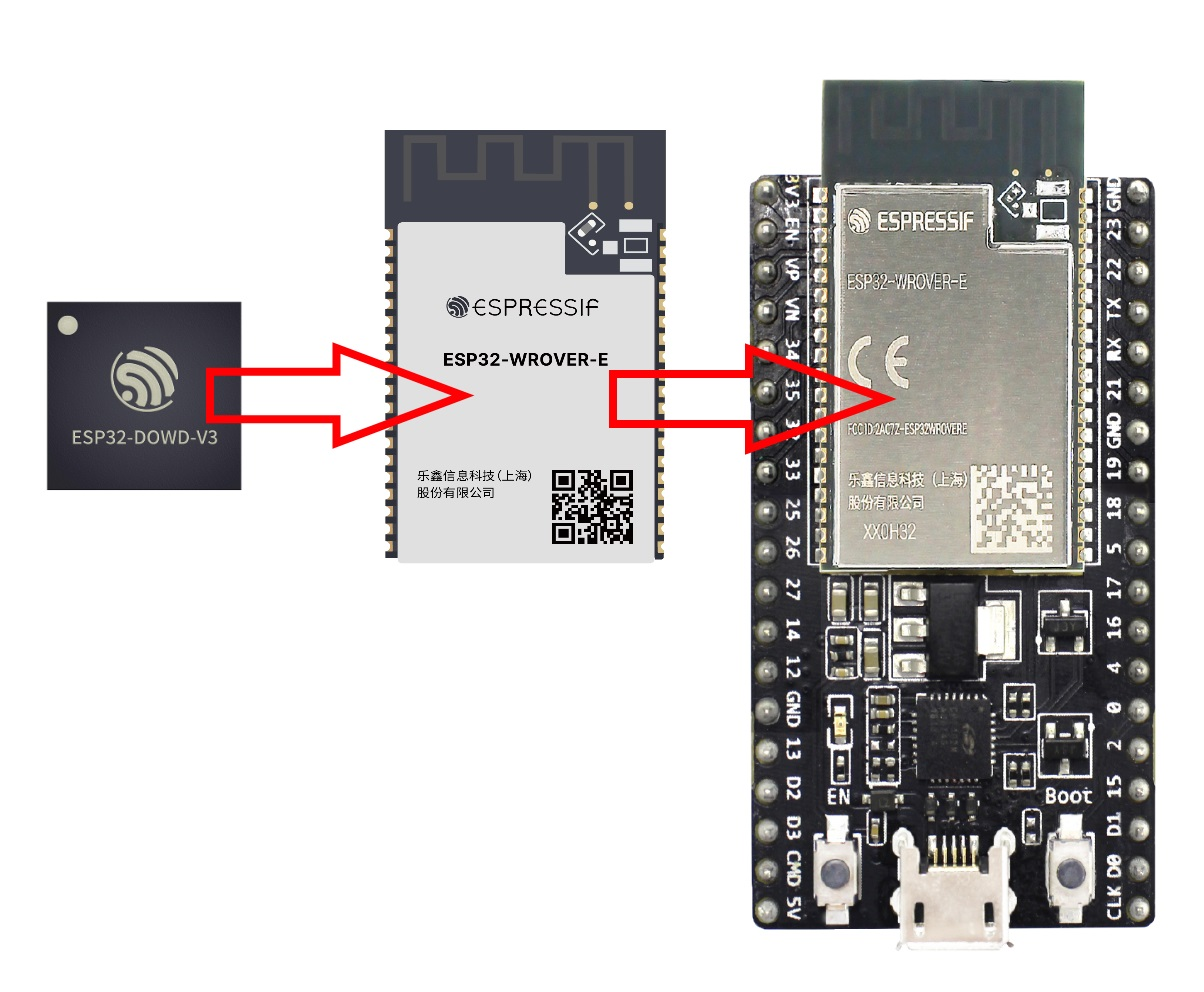
\includegraphics[scale=0.4]{placa_modulo_soc}
  \caption{De izquierda a derecha: sistema en chip, módulo de la serie ESP32 y placa de desarrollo de la serie ESP32.}\label{fig:placa_modulo_soc}
\end{figure}

La serie de kits de desarrollo que se ajusta a los requisitos de selección es la ESP32 ya que soporta WiFi, Bluetooth y BLE. Dentro de esta serie, es necesario descartar todas aquellas placas orientadas a procesamiento digital de señales, procesamiento de audio y vídeo, reconocimiento de voz y demás características que no son necesarias para la prótesis híbrida. Se desea además una placa de desarrollo de tamaño reducido para su fácil integración en la estructura de la prótesis.
\\
\\
Dentro de la serie mencionada, quedan entonces dos opciones: el ESP32-DevKitC y el ESP32-PICO-KIT. La segunda de estas dos placas es la más pequeña con un tamaño de 52 x 20.3 mm\cite{picokit}. Sin embargo, no tiene ningún tipo de antena integrada lo cual requiere un análisis de la más adecuada, su adquisición, instalación y comprobación de su correcto funcionamiento. Se descarta esta placa de desarrollo ya que la ESP32-DevKitC es la que más se ajusta a los requisitos de selección, tiene antena integrada en la tarjeta de circuito impreso y su tamaño no es mucho mayor que el de la ESP32-PICO-KIT con unas medidas de 54.4 x 27.9 mm\cite{devkitc}.
\\
\\
Una vez seleccionada la placa de desarrollo ESP32-DevKitC, se ha de determinar cuál de sus posibles módulos es el más adecuado para la prótesis híbrida. Para ello se lleva a cabo un análisis de los módulos disponibles en la tablas \ref{tabla:modulos_esp32_1} y \ref{tabla:modulos_esp32_2}.
\\
\\
Analizando estas tablas, se aprecia en primer lugar que hay tres módulos que no tienen la antena integrada sino un conector para que el usuario acople una. Al igual que el caso del ESP32-PICO-KIT, se descartan estos módulos por el motivo ya explicado. Además, no es necesaria una transmisión de datos inalámbrica a larga distancia o con obstáculos en el camino ya que los componentes de la prótesis estarán cercanos entre sí. Por lo tanto, la antena integrada es la mejor opción.
\\
\\
Otro punto en el que difieren los módulos resultantes es su CPU. El ESP32-WROOM-32E y el ESP32-WROVER-E tienen una CPU de dos núcleos mientras que la del ESP32-SOLO-1 tiene uno. Esto implica que la opción de dos núcleos consume más energía. De hecho, en la tabla \ref{tabla:modulos_esp32_1} se aprecia un consumo máximo de casi el doble por parte de la CPU de dos núcleos en comparación con la de uno. Sin embargo, este consumo es el que se produce a la velocidad de reloj máxima: 240MHz para la CPU de dos núcleos y 160MHz para la de uno. Cuando esta velocidad se reduce a 80MHZ, lo cual es lo más probable para la aplicación del presente trabajo, los consumos de ambas CPUs son prácticamente iguales\cite{esp32_consumo_cpu}. Por tanto, se elige la CPU de dos núcleos ya que aporta más versatilidad y potencia de procesamiento con un consumo similar a la CPU de un núcleo para la configuración de velocidad de reloj ya explicada.
\\
\\
Solamente queda elegir entre los módulos ESP32-WROOM32-E y ESP32-WROVER-E. Su principal diferencia es la RAM: el primero tiene 520KB on chip mientras que el segundo tiene además 8MB de Pseudo SRAM o PSRAM. Los requisitos de selección del microcontrolador no especifican un manejo ni almacenamiento de datos considerable por lo que no se requiere una SRAM excesivamente grande. En consecuencia, se descarta el módulo ESP32-WROVER-E puesto que no es necesario tener la memoria RAM sobredimensionada.
\\
\\
Se muestra en la imagen \ref{fig:seleccion_placa} la placa de desarrollo seleccionada: ESP32-DevKitC-32E.

\begin{figure}[!htb]
\centering
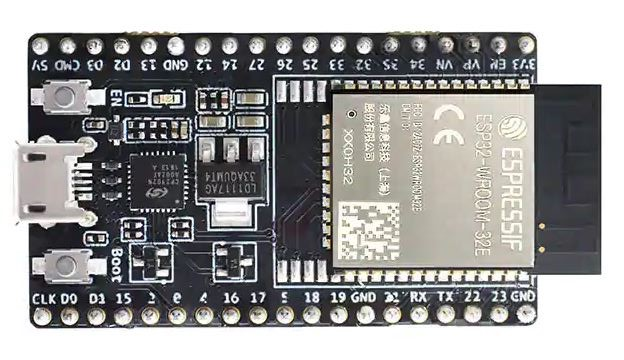
\includegraphics[scale=0.5]{seleccion_placa}
  \caption{Placa de desarrollo Espressif ESP32-DevKitC-32E.}\label{fig:seleccion_placa}
\end{figure}

\begin{landscape}

\begin{table}[]
\centering
\begin{tabular}{|c|c|c|c|c|c|c|}
\hline
\begin{tabular}[c]{@{}c@{}}Placa \\ de desarrollo\end{tabular} & Módulo                                & Antena                            & CPU                                                                                                         & \begin{tabular}[c]{@{}c@{}}Consumo \\ máximo CPU\cite{esp32_consumo_cpu}\end{tabular}                       & FLASH                & RAM                                                                      \\ \hline
\multirow{6}{*}{ESP32-DevKitC}                                 & ESP32-SOLO-1                          & \multirow{3}{*}{Integrada}        & \begin{tabular}[c]{@{}c@{}}ESP32-S0WD \\ Single Core\\ 32 bits\\ 160MHz max.\end{tabular}                   & \begin{tabular}[c]{@{}c@{}}34mA a 3,3V\\ 112mW aprox.\end{tabular}                  & \multirow{3}{*}{4MB} & \multirow{2}{*}{\begin{tabular}[c]{@{}c@{}}520KB\\ on chip\end{tabular}} \\ \cline{2-2} \cline{4-5}
                                                               & ESP32-WROOM-32E                       &                                   & \multirow{2}{*}{\begin{tabular}[c]{@{}c@{}}ESP32-D0WD-V3 \\ Dual Core\\ 32 bits\\ 240MHz max.\end{tabular}} & \multirow{2}{*}{\begin{tabular}[c]{@{}c@{}}68mA a 3,3V\\ 225mW aprox.\end{tabular}} &                      &                                                                          \\ \cline{2-2} \cline{7-7} 
                                                               & ESP32-WROVER-E                        &                                   &                                                                                                             &                                                                                     &                      & \begin{tabular}[c]{@{}c@{}}520KB\\ on chip\\ 8MB\\ PSRAM\end{tabular}    \\ \cline{2-7} 
                                                               & \multicolumn{1}{l|}{ESP32-WROOM-32U}  & \multicolumn{1}{l|}{No integrada} & -                                                                                                           & -                                                                                   & -                    & -                                                                        \\ \cline{2-7} 
                                                               & \multicolumn{1}{l|}{ESP32-WROOM-32UE} & \multicolumn{1}{l|}{No integrada} & -                                                                                                           & -                                                                                   & -                    & -                                                                        \\ \cline{2-7} 
                                                               & \multicolumn{1}{l|}{ESP32-WROVER-IE}  & \multicolumn{1}{l|}{No integrada} & -                                                                                                           & -                                                                                   & -                    & -                                                                        \\ \hline
\end{tabular}
\caption{Comparación de módulos de la serie ESP32\cite{modulos_esp32}.}
\label{tabla:modulos_esp32_1}
\end{table}

\begin{table}[]
\centering
\begin{tabular}{|c|c|c|c|c|c|c|c|}
\hline
\begin{tabular}[c]{@{}c@{}}Placa \\ de desarrollo\end{tabular} & Módulo                                & SPI                 & I2C                 & UART                & Bluetooth                                                                 & WiFi                                                                                        & \begin{tabular}[c]{@{}c@{}}Precio \\ unitario\end{tabular} \\ \hline
\multirow{6}{*}{ESP32-DevKitC}                                 & ESP32-SOLO-1                          & \multirow{3}{*}{x2} & \multirow{3}{*}{x2} & \multirow{3}{*}{x3} & \multirow{3}{*}{\begin{tabular}[c]{@{}c@{}}Bluetooth \\ BLE\end{tabular}} & \multirow{3}{*}{\begin{tabular}[c]{@{}c@{}}IEEE \\ 802.11b/g/n\\ 150Mbps max.\end{tabular}} & \multirow{3}{*}{8€}                                        \\ \cline{2-2}
                                                               & ESP32-WROOM-32E                       &                     &                     &                     &                                                                           &                                                                                             &                                                            \\ \cline{2-2}
                                                               & ESP32-WROVER-E                        &                     &                     &                     &                                                                           &                                                                                             &                                                            \\ \cline{2-8} 
                                                               & \multicolumn{1}{l|}{ESP32-WROOM-32U}  & -                   & -                   & -                   & -                                                                         & -                                                                                           & -                                                          \\ \cline{2-8} 
                                                               & \multicolumn{1}{l|}{ESP32-WROOM-32UE} & -                   & -                   & -                   & -                                                                         & -                                                                                           & -                                                          \\ \cline{2-8} 
                                                               & \multicolumn{1}{l|}{ESP32-WROVER-IE}  & -                   & -                   & -                   & -                                                                         & -                                                                                           & -                                                          \\ \hline
\end{tabular}
\caption{Comparación de módulos de la serie ESP32\cite{modulos_esp32}.}
\label{tabla:modulos_esp32_2}
\end{table}

\end{landscape}



\section{Implementación de los protocolos de comunicación}
Una vez seleccionada la placa de desarrollo ESP32-DevKitC-32E como nodo central de la prótesis, se han de determinar los protocolos de comunicación entre este dispositivo y el resto de los componentes de la misma. Se va a proceder en primer lugar al análisis de los protocolos disponibles para cada componente para continuar con su comparación y finalmente seleccionar los más óptimos.

\subsection{Protocolo con el exoesqueleto}
\subsection{Protocolo con la interfaz}
\subsection{Protocolo con los estimuladores eléctricos}

Se revisa la configuración establecida en el USART1. En primer lugar se aprecia que el Registro C de Configuración y Estado del USART1 contiene el siguiente valor:\\

\begin{lstlisting}[language=C++,breaklines]
UCSR1C = 0x86;
\end{lstlisting}

Esta configuración, según la hoja de datos del microcontrolador, establece los siguientes ajustes en la comunicación serial por USART:

\begin{itemize}
\item[•] Modo de operación asíncrono.
\item[•] Modo de paridad deshabilitado.
\item[•] Un bit de parada.
\item[•] Ocho bits para datos.
\end{itemize}
 
El modo de operación es en efecto asíncrono, lo que quiere decir que los dispositivos conectados al estimulador por puerto serie no se comunican mediante una línea de datos y un reloj compartido. En cambio, como ya se ha visto anteriormente, existe una línea de transmisión y otra de recepción de datos. Por tanto, los dispositivos a ambos extremos de estas líneas deben conocer las características de la comunicación serial. Esto es así porque el estimulador originalmente se comunica de forma inalámbrica lo que imposibilita compartir una línea de reloj con el dispositivo al que se conecta. En cuanto al tamaño de los datos, se utiliza 8 bits por cuestiones de compatibilidad con los dispositivos conectados al microcontrolador.
\\
\\
Por otra parte, observando el valor del registro A de control y estado del USART1 se aprecia que está configurado de la siguiente manera: 

\begin{lstlisting}[language=C++,breaklines]
UCSR1A = 0X02;
\end{lstlisting}

En esta configuración se tiene el segundo bit de dicho registro a un valor de 1 lo que implica la activación de la funcionalidad de doble velocidad para comunicaciones asíncronas. Se muestra en la figura \ref{fig:U2X_datasheet} dicha configuración según la hoja de datos del ATmega128L.\\

\begin{figure}[!htb]
\centering
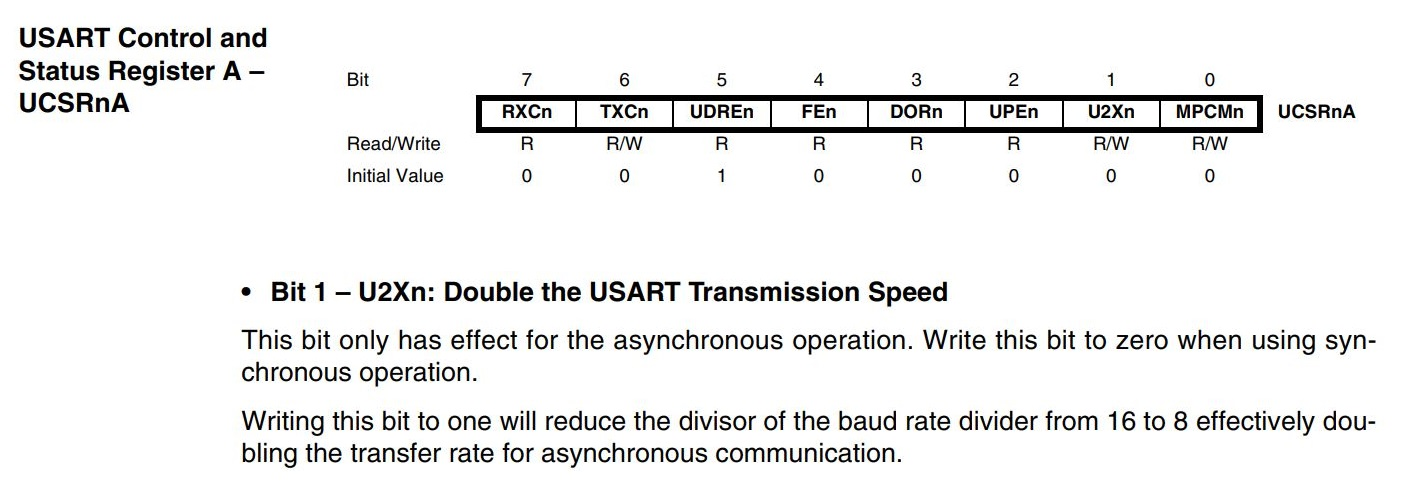
\includegraphics[scale=0.45]{U2X_datasheet}
  \caption{Descripción del modo de doble velocidad en comunicaciones asíncronas para el ATmega128L según su hoja de datos.}\label{fig:U2X_datasheet}
\end{figure}

Por otro lado, se tienen los registros de configuración de tasa de baudios UBRR1H y UBRR1L en los cuales que se carga el valor contenido en $ubrr$ según la siguiente configuración efectuada en la función de inicialización del USART1:\\

\begin{lstlisting}[language=C++,breaklines]
UBRR1H = (unsigned char)(ubrr>>8);
UBRR1L = (unsigned char)ubrr;
\end{lstlisting}

A partir de ahora se hablará de la velocidad de comunicación en bits por segundo por cuestiones de homogeneidad en la terminología. Se ha tomado esta decisión ya que bits por segundo y baudios no so lo mismo aunque se usen indistintamente de forma extendida.
\\
\\
Teniendo en cuenta el modo de doble velocidad explicado previamente, la frecuencia de reloj del microcontrolador de $8MHz$, y que el valor de $ubrr$ observado en el firmware es de 8, la figura \ref{fig:UBRR_datasheet} obtenida de la hoja de datos muestra que se tiene una velocidad de comunicación USART asíncrona de 115200 bps.\\

\begin{figure}[!htb]
\centering
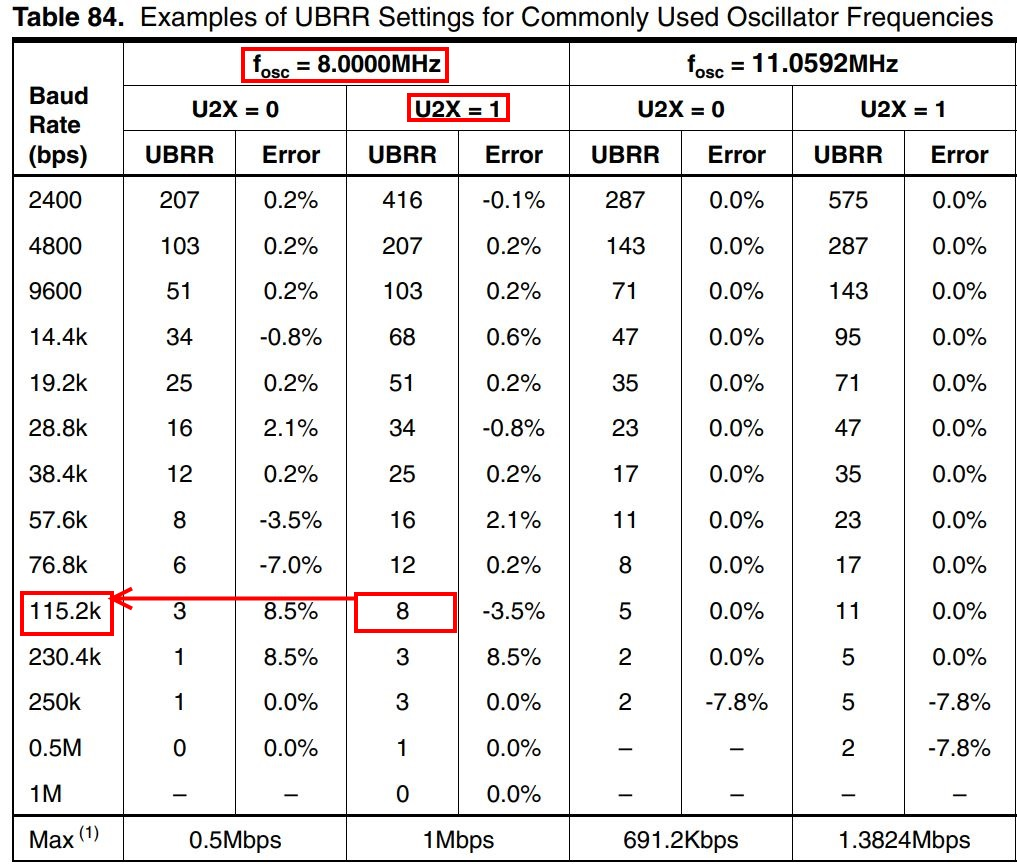
\includegraphics[scale=0.4]{UBRR_datasheet}
  \caption{Valores del registro de tasa de baudios según la velocidad de reloj y la modalidad de doble velocidad. Se indican en rojo los valores observados en el firmware original del mini TEREFES.}\label{fig:UBRR_datasheet}
\end{figure}

Una vez vista la configuración del USART1 del que se sirve el microcontrolador para comunicarse, se concluye que los factores que se pueden modificar para optimizar la comunicación son su velocidad en bits por segundo, los bits de parada y la paridad de bits. Trabajando con el estimulador se ha observado que una velocidad de 115200bps puede ser demasiado elevada en una aplicación como la que concierne al electroestimulador ya que no se requiere la transmisión de grandes cantidades de datos. Además, ciertas velocidades conllevan probabilidades de errores más elevadas tal y como indica la hoja de datos del ATmega128L en la figura \ref{fig:UBRR_datasheet}. Esto afecta a la integridad de los mensajes y por tanto a la efectividad del estimulador en su asistencia.

Se ha intentado establecer comunicación con el módulo de comunicación inalámbrica del dispositivo desde un ordenador mediante un puerto serie virtual y Bluetooth. Para ello se ha escrito un script en Python el cual se encarga de transmitir comandos al mini TEREFES de la siguiente forma:


\begin{lstlisting}[language=C++,breaklines]
import pyserial

puerto_serie = serial.Serial(
	port = 'COM3',
	baudrate = 115200,
	parity = serial.PARITY_NONE,
	stopbits = serial.STOPBITS_ONE,
	bytesize = serial.EIGHBITS,
	timeout = 2
)

comando = "w 0 ap 30\r"

if puerto_serie.is_open:
	for c in comando:
		puerto_serie.write(c.encode())
		
	if puerto_serie.inWaiting() > 0:
		print(puerto_serie.read().decode())	
\end{lstlisting}

Con este script se establece comunicación con el electroestimulador mediante un puerto serie virtual $COM3$. Entonces, envía a éste el comando ``w 0 ap 30\textbackslash r'' visto con anterioridad y a continuación se recibe por el mismo puerto serie la respuesta del mini TEREFES, pues para esta prueba se ha configurado el firmware para que devuelva los mensajes que recibe. El resultado es la devolución de mensajes incompletos o incoherentes por parte del estimulador indicando una velocidad de comunicación inadecuada. Para corroborar esto, se modifica dicha velocidad para que resulte en 19200 bps, un valor de 51 en el registro UBRR según la figura \ref{fig:UBRR_datasheet} y se observa que los mensajes llegan adecuadamente. 

\subsubsection{USART mediante cable}
Para establecer este tipo de comunicación solamente son necesarios tres cables para formar las líneas de transmisión y recepción de datos y unir las masas de los dispositivos conectados. En la imagen representativa de la placa de control mostrada en el Anexo 1, el conector JP5 es el encargado de la comunicación. Para ello se sirve de cuatro alojamientos en los que alojar cables o el módulo Bluetooth ya visto y que se tratará más adelante. De este modo, se utilizan los alojamientos 2, 3 y 4 del conector JP5 que son la referencia a masa, la línea de transmisión del estimulador y la de recepción, respectivamente.

\subsubsection{USART mediante Bluetooth y BLE}
Para establecer comunicación inalámbrica con el estimulador hay que alojar el módulo Bluetooth en el conector JP5 de la placa de control. Una vez hecho esto, es posible conectarse a dicho módulo desde cualquier dispositivo con Bluetooth y capacidad de comunicación serial. Esto se puede conseguir con un ordenador con Bluetooth y una terminal de puerto serie tal y como se indicó en el capítulo \ref{capitulo_2}.
\\
\\
Para el ajuste de velocidad de comunicación, hay que llevar a cabo lo descrito en el apartado anterior dedicado a la comunicación cableada, esto es, ajustar la velocidad del USART en el mcicrocontrolador.
\\
\\
El siguiente paso es ajustar la velocidad de comunicación en el módulo Bluetooth, para lo cual es útil la documentación ofrecida en la página web del producto. Las herramientas necesarias para esta tarea son el propio módulo Bluetooth Sparkfun Silver Smirf y un Arduino Uno.
\\
\\
En primer lugar se ha de conectar el módulo Bluetooth al Arduino de la manera indicada en la figura \ref{fig:configuracion_modulos_BT}. En cuanto al programa para la configuración del módulo, se utiliza el sugerido por Sparkfun y el cual se muestra a continuación:


\begin{lstlisting}[language=C++,breaklines]
/*
  Example Bluetooth Serial Passthrough Sketch
 by: Jim Lindblom
 SparkFun Electronics
 date: February 26, 2013
 license: Public domain

 This example sketch converts an RN-42 bluetooth module to
 communicate at 9600 bps (from 115200), and passes any serial
 data between Serial Monitor and bluetooth module.
 */
#include <SoftwareSerial.h>  

int bluetoothTx = 2;  // TX-O pin of bluetooth mate, Arduino D2
int bluetoothRx = 3;  // RX-I pin of bluetooth mate, Arduino D3

SoftwareSerial bluetooth(bluetoothTx, bluetoothRx);

void setup()
{
  Serial.begin(9600);  // Begin the serial monitor at 9600bps

  bluetooth.begin(115200);  // The Bluetooth Mate defaults to 115200bps
  bluetooth.print("$");  // Print three times individually
  bluetooth.print("$");
  bluetooth.print("$");  // Enter command mode
  delay(100);  // Short delay, wait for the Mate to send back CMD
  bluetooth.println("U,9600,N");  // Temporarily Change the baudrate to 9600, no parity
  // 115200 can be too fast at times for NewSoftSerial to relay the data reliably
  bluetooth.begin(9600);  // Start bluetooth serial at 9600
}

void loop()
{
  if(bluetooth.available())  // If the bluetooth sent any characters
  {
    // Send any characters the bluetooth prints to the serial monitor
    Serial.print((char)bluetooth.read());  
  }
  if(Serial.available())  // If stuff was typed in the serial monitor
  {
    // Send any characters the Serial monitor prints to the bluetooth
    bluetooth.print((char)Serial.read());
  }
  // and loop forever and ever!
}
\end{lstlisting}

Este programa establece comunicación con el módulo Bluetooth mediante las conexiones en los pines 2 y 3 del Arduino. Lo hace a una velocidad de 9600bps, considerando que la que trae por defecto el módulo es de 115200bps. Una vez cargado, se abre la terminal serie de Arduino y utilizando los comandos de configuración del módulo adecuados, se ajusta la velocidad a la que se va a comunicar. Estos comandos se encuentran también en la web del producto y los necesarios para la tarea que se está tratando son:

\begin{itemize}
\item[•] \$\$\$: Entrada al modo de configuración. Antes de modificar los parámetros del módulo Bluetooth, es necesario ponerlo en el estado de configuración. 
\item[•] SU,<valor>: Este comando permite modificar la velocidad de comunicación del dispositivo en bits por segundo. Los posibles valores son 1200, 2400, 4800, 9600, 19.2, 28.8, 38.4, 57.6, 115K, 230K, 460K, or 921K. Solamente es necesario especificar los dos primeros dígitos por lo que si se desea una velocidad de 115200bps se ha de introducir ``SU,11''.
\item[•] ---: Salir del modo de configuración. Tras introducir este comando el módulo volverá a su funcionamiento normal.
\end{itemize}

\begin{figure}[!htb]
\centering
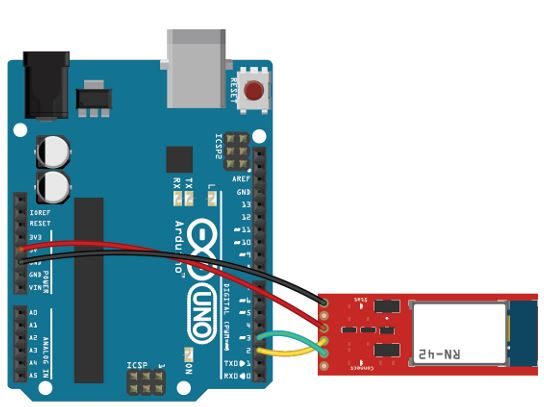
\includegraphics[scale=0.6]{configuracion_modulos_BT}
  \caption{Conexión del módulo Bluetooth al Arduino para su configuración. La línea de transmisión de datos del módulo se conecta a la de recepción del Arduino, es decir el pin 2. La línea de recepción de datos del módulo Bluetooth se conecta a la de transmisión del Arduino, el pin 3.}\label{fig:configuracion_modulos_BT}
\end{figure}

Al igual que el caso de la comunicación cableada, el dispositivo que se conecta al microcontrolador, en este caso mediante el módulo Bluetooth, debe tener la misma velocidad de comunicación serial que estos dos dispositivos.


\subsubsection{Pruebas de velocidad y selección del protocolo}
pruebas cable vs BT de respuesta fisica y devolver datos con parametros baud rate y codificacion o no

PARAMETROS USART1
Los parámetros del USART1 que se van a modificar son los siguientes:

\begin{itemize}
\item[•] Velocidad de comunicación en bits por segundo.
\item[•] Bits de parada.
\item[•] Paridad de bits.
\end{itemize}

Para modificar la velocidad de comunicación solamente es preciso guardar en los registros UBRRH1 y UBRRL1, los cuales forman el UBRR, los valores correspondientes para cada velocidad, según indica la hoja de datos del microcontrolador. Hay que tener en cuenta que la velocidad del reloj del sistema es de $8MHz$ y que el modo de doble velocidad (U2X) está activado. Esto implica, según la figura \ref{fig:UBRR_datasheet} que las posibles velocidades de comunicación por USART y sus respectivos valores de los registros mencionados son los mostradas en la tabla \ref{tabla:velocidades_USART}.\\

\begin{table}
\centering
\begin{tabular}{| p{20mm} | p{30 mm} |}
\hline
\textbf{UBRR} & \textbf{Velocidad (bps)} \\ \hline
416 & 2400\\ \hline
207 & 4800\\ \hline
103 & 9600\\ \hline
68 & 14400\\ \hline
51 & 19200\\ \hline
34 & 28800\\ \hline
25 & 38400\\ \hline
16 & 57600\\ \hline
12 & 76800\\ \hline
8 & 115200\\ \hline
3 & 230400\\ \hline
3 & 250000\\ \hline
1 & 500000\\ \hline
0 & 1000000\\ \hline
\end{tabular}\caption{Valores del registro de tasa de baudios del USART del ATmega128L para un reloj de $8MHz$ y modo de doble velocidad activado (U2X =1) en USART asíncrono.}\label{tabla:velocidades_USART}
\end{table}

Para modificar los bits de parada y la paridad de bits se utiliza el Registro C de Control y Estado tal y como se muestra en la figura \ref{fig:UCSRNC_datasheet}. Los bits 5 y 4 de este registro ofrecen la posibilidad dedeshabilitar la paridad de bits o utilizar un bit de paridad par o impar. El bit 3 del registro de configuración permite configurar uno o dos bits de parada.\\

\begin{figure}[!htb]
\centering
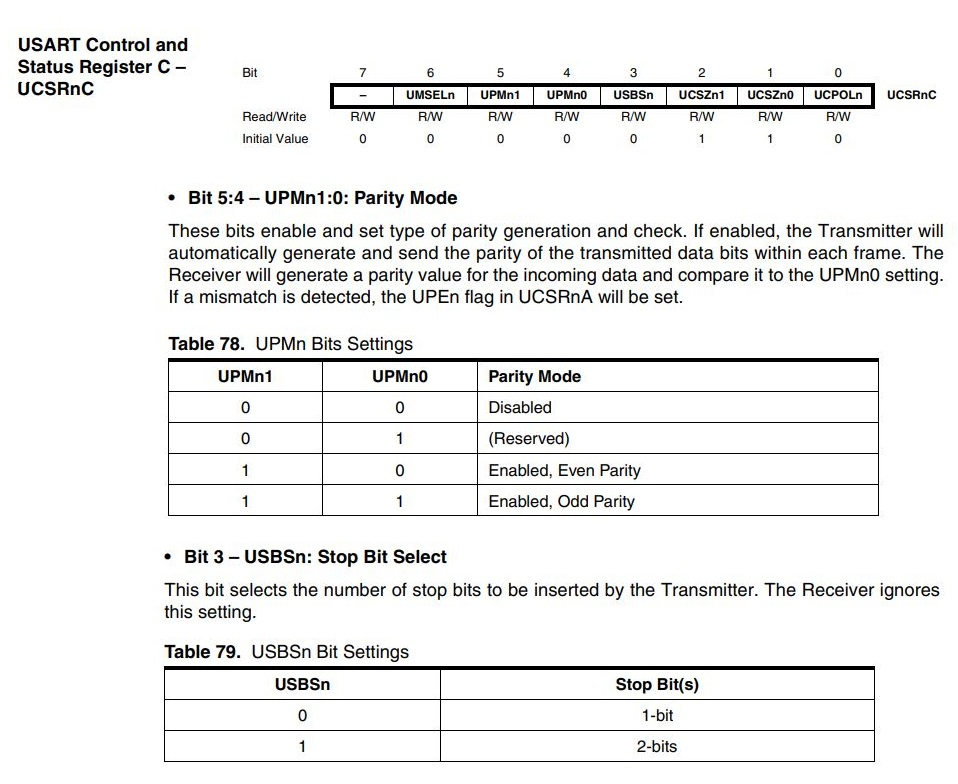
\includegraphics[scale=0.6]{UCSRNC_datasheet}
  \caption{Configuración de la paridad de bits y los bits de parada en el Registro C de Control y Estado del USART.}\label{fig:UCSRNC_datasheet}
\end{figure}


\section{Programación del microcontrolador}
\subsection{Interfaz gráfica}
\subsection{Exoesqueleto robótico}
\subsection{Estimuladores eléctricos}
